\documentclass[letter]{article}
\usepackage[monocolor]{../math232/ahsansabit}
\usepackage[]{float}
\title{Quantum Mechanics : : Homework 03}
\author{Ahmed Saad Sabit, Rice University}
\date{\today}

\begin{document}
\maketitle

\section*{Problem 01} 
\subsection*{(a)}
I did the first matrix multiplication computation by hand and it aligns with what I got from Matlab. There's way too many multiplication to do so I am instead opting for matlab solution. 

\[
\sigma_1 \kappa_1 = 
\begin{pmatrix} 0&0&0&1\\0&0&1&0\\0&1&0&0\\1&0&0&0 \end{pmatrix} 
\] 
\[
\kappa_1 \sigma_1 = \begin{pmatrix} 0&0&0&1\\0&0&1&0\\0&1&0&0\\1&0&0&0 \end{pmatrix} 
\]
I have thought enough how to convince the grader that I know how to do Matrix Multiplication, the most tedious approach being I show each and every single individual dot product on paper. That's too much work. 

We just wanna prove that the commutator is zero
\[
	[ \sigma_1 \kappa_1 ] = 
	\sigma_1 \kappa_1 - \kappa_1 \sigma_1 = 0
\]

Very similarly we can keep doing it, one by one in MATLAB 

\begin{figure}[H]
	\centering
	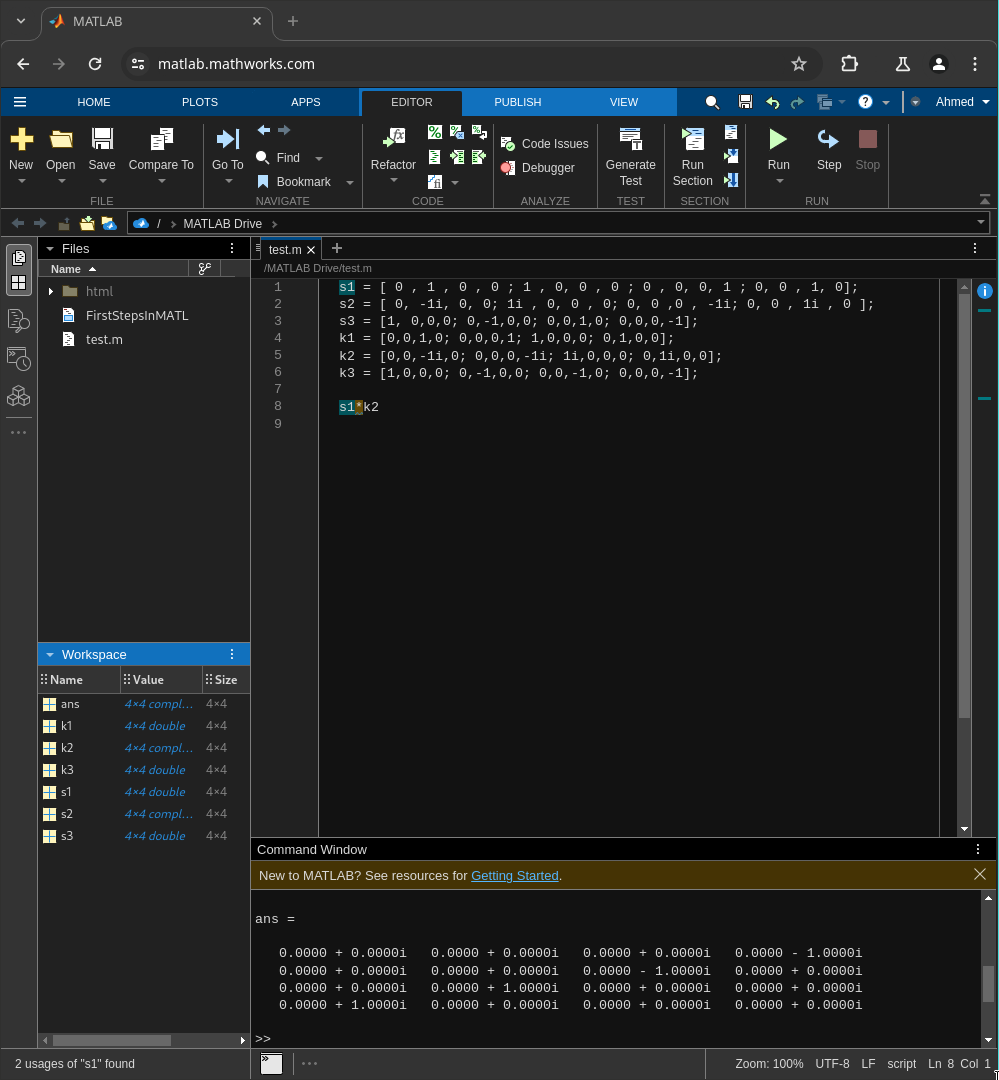
\includegraphics[width=0.6\textwidth]{ss/matlab01.png}
	\caption{Computing $\sigma_1 \kappa_2$}
	\label{fig:ss-matlab01-png}
\end{figure}

We find 
\[
\sigma_1 \kappa_2 = \kappa_2 \sigma_1 
=\begin{pmatrix} 0&0&0&-i\\0&0&-i&0\\0&i&0&0\\i&0&0&0 \end{pmatrix} 
\quad 
\to \quad [\sigma_1, \kappa_2] = 0\]

\[
\sigma_1 \kappa_3 = \kappa_3 \sigma_1 = 
\begin{pmatrix} 0&1&0&0\\1&0&0&0\\0&0&0&-1\\0&0&-1&0 \end{pmatrix} 
\quad \to \quad [\sigma_1, \kappa_3]=0 \] 

\[
\sigma_2 \kappa_2 = \kappa_2 \sigma_2 = 
\begin{pmatrix} 0&0&0&-1\\0&0&1&0\\0&1&0&0\\-1&0&0&0 \end{pmatrix}  
\quad \to \quad [\sigma_2, \kappa_2] = 0
\]

\[
\sigma_2 \kappa_3 = \kappa_3 \sigma_2 = 
\begin{pmatrix} 0&-i&0&0\\i&0&0&0\\0&0&0&i\\0&0&-i&0  \end{pmatrix}  
\quad \to \quad [\sigma_2, \kappa_3] = 0
\]

\newpage
\subsection*{b}
Take $\sigma_1$ and do pen and paper calculation to find out the eigenvalues. I used mathematica to find out the determinant safely and we get the eigenvalues from the characteristic polynomial
\[
\lambda^{4} - 2 \lambda^2 + 1 = 0
\]
Which gives, 
\[
\lambda = -1, -1, 1, 1
\]
Set of eigenvectors for $\sigma_1$ being 
\[
\begin{pmatrix} 0\\0\\-1\\1 \end{pmatrix} , 
\begin{pmatrix} -1\\1\\0\\0 \end{pmatrix} ,
\begin{pmatrix} 0\\0\\1\\1 \end{pmatrix} ,
\begin{pmatrix} 1\\1\\0\\0 \end{pmatrix} 
\]

Now let's do this for the $\kappa_2$ and we get the characteristic equation
\[
\lambda^{4} - 2 \lambda^2 + 1
\] 
And we get 
\[
\lambda = -1,-1,1,1
\] 
With Eigenvectors
\[
\begin{pmatrix} 0\\i\\0\\1 \end{pmatrix} 
,
\begin{pmatrix} i\\0\\1\\0 \end{pmatrix} ,
\begin{pmatrix} 0\\-i\\0\\1 \end{pmatrix} ,
\begin{pmatrix} -i\\0\\1\\0 \end{pmatrix} 
\] 
By theory if there are common eigenvectors, 
\[
A | \phi \rangle  = \phi_A | \phi \rangle 
\] 
\[
B | \phi \rangle  = \phi_B | \phi \rangle 
\] 
Then
\[
AB | \phi \rangle  = \phi_A \phi_B | \phi \rangle 
\]
Taking $\sigma_1 \kappa_2$, 
\[
\sigma_1 \kappa_2 = 
\begin{pmatrix} 0&0&0&-i\\0&0&-i&0\\0&i&0&0\\i&0&0&0 \end{pmatrix} 
\] 
The eigenvectors of these are 
\[
\begin{pmatrix} i\\0\\0\\1 \end{pmatrix} ,
\begin{pmatrix} 0\\i\\1\\0 \end{pmatrix} ,
\begin{pmatrix} -i\\0\\0\\1 \end{pmatrix} ,
\begin{pmatrix} 0\\-i\\1\\0 \end{pmatrix} 
\]
Looking at the eigenvectors we know there are NO common eigenvectors.

\newpage
\section*{Problem 02} 
\subsection*{a} 
Total force on $m_1$ and $m_2$
\[
	m_1 \ddot{x}_1 = - k_A x_1 + k_B (x_2 - x_1) 
\]
\[
	m_2 \ddot{x} _2 = - k_B(x_2 - x_1) + k_C(L - x_2 - x_1)
\]
The equilibriums are for which net force is zeroed 
\[
0 = - k_A x_1 + k_B (x_2 - x_1) 
\]
\[
0 = - k_B(x_2 - x_1) + k_C(L - x_2 - x_1)
\]
Trying to solve this by hand I get, 
\[
x_1 = \frac{k_B}{k_A + k_B} x_2
\]
Individual solution 
\[
x^{0}_2 = \frac{k_A k_C + k_B k_C}{(k_B+k_C)(k_A + k_B) - (k_B-k_C) k_B} L
\]
\[
x^{0}_1 = \frac{k_B k_C }{(k_B + k_C)(k_A+k_B) - (k_B - k_C)k_B} L 
\]
\begin{figure}[H]
	\centering
	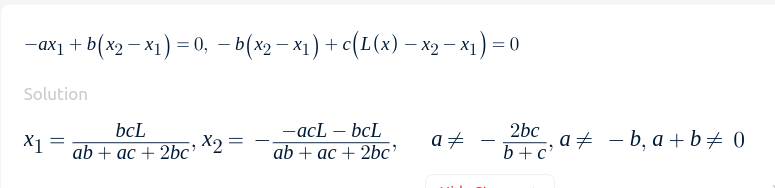
\includegraphics[width=0.8\textwidth]{ss/symbogimbo.png}
	\caption{Verifying that I haven't really messed up.}
	\label{fig:ss-symbogimbo-png}
\end{figure}

\subsection*{b} 
Apparently $\ddot x_i = \delta \ddot{x}_i $. And
\[
x_2 - x_1 = x_2^{0 } - x_1^{0} + \delta x_2 - \delta x_1 
\]
As we know the denominator of $x_1^{0}, x_2^{0}$ are the same, calling them as $D$, 
\[
x_2 - x_1 = \frac{k_A k_C L}{D} + \delta x_2 - \delta x_1 
\] 
\[
x_2 + x_1 = \frac{k_A k_C + 2 k_B k_C}{D } L + \delta x_1 + \delta x_2 
\] 
Thus through substituting our new formulas for $x_2-x_1$ and $x_1+x_2$ with equilibrium position in the newton's equations we can get, 
\[
m_1 \delta \ddot x_1 = - \frac{k_A k_B k_C L}{D} - k_A \delta x_1  + \frac{k_A k_B k_C L}{D} + k_B (\delta x_2 - \delta x_1) = \boxed{
  -k_A \delta x_1 + k_B (\delta x_2 - \delta x_1)
}\]
For the second equation, 
\[
m_2 \delta \ddot x_2 = - \frac{k_A k_B k_C L}{D} - k_B (\delta x_2 - \delta x_1) + k_C L -\frac{k_A k_C^2 L+ 2 k_B k_C^2L}{D}   - k_C (\delta d x_2 + \delta d x_1)
\]  

\[
m_2 \delta \ddot x_2 = - \frac{k_A k_B k_C L}{D} - k_B (\delta x_2 - \delta x_1) + \frac{ k_C D L - k_A k_C^2 L- 2 k_B k_C^2L}{D}  +k_C L  - k_C (\delta d x_2 + \delta d x_1)
\] 

Note that $D = (k_B + k_C)(k_A +k_B) - (k_B - k_C) k_B =  k_A k_B + k_A k_C + 2 k_B k_C$, hence
\[
\frac{k_C D L - k_A k_C^2 L - 2 k_B k_C^2 L }{D} = 
\frac{k_A k_B k_C + k_A k_C^2 + 2 k_B k_C^2 - k_A k_C^2 - 2 k_B k_C^2 }{D} L = \frac{k_A k_B k_C}{D} L 
\]


\[
m_2 \delta \ddot x_2 = - \frac{k_A k_B k_C L}{D} - k_B (\delta x_2 - \delta x_1) + \frac{ k_A k_B k_C	}{D}L +k_C L   - k_C (\delta d x_2 + \delta d x_1)
\]
With $m_1 = m_2 = m$, we finalize 
\[
\boxed{
m \delta \ddot x_2 = -k_B (\delta x_2 - \delta x_1)  - k_C  \delta x_2 
} \] 

\[
\boxed{
m \delta \ddot x_1 = - k_A \delta x_1 + k_B (\delta x_2 - \delta x_1)
}
\] 

\subsection*{c} 
We can divide both sides of equations with $m$ and name $k_I / m = \omega_I^2$
\[
 \delta \ddot x_1 = - \omega_A^2 \delta x_1 + \omega_B^2 (\delta x_2 - \delta x_1) 
\] 
\[
 \delta \ddot x_2 = -\omega^2_B (\delta x_2 - \delta x_1)  - \omega^2_C  \delta x_2 
 \] 
The homogenous set of equation, 

 \begin{align*}
	 \delta \ddot x_1 &= (-\omega^2_A - \omega^2_B ) \delta x_1 + \omega_B^2 \delta x_2  \\
	 \delta \ddot x_2 &=\omega^2_B   \delta x_1 + (- \omega_B^2 - \omega_C^2 ) \delta x_2 \\
 \end{align*}
This is very equivalently
\[
\begin{pmatrix} \delta \ddot x_1 \\ \delta \ddot x_2 \end{pmatrix}  = 
\begin{pmatrix}  (-\omega^2_A - \omega^2_B ) & \omega_B^2 \\
	\omega^2_B & (- \omega_B^2 - \omega_C^2 ) 
\end{pmatrix}
\begin{pmatrix} \delta x_1 \\ \delta x_2 \end{pmatrix} 
\]
Simplify notation to avoid myself to getting hospitalized. 
\[
\begin{pmatrix} \delta \ddot x_1 \\ \delta \ddot x_2 \end{pmatrix}  = 
\begin{pmatrix}  -A-B  & B \\
	B & -B - C  
\end{pmatrix}
\begin{pmatrix} \delta x_1 \\ \delta x_2 \end{pmatrix} 
\]
The characteristic equation is 
\[
\frac{1}{m^2}	(k_A k_B + k_A k_C + k_B k_C) + \frac{1}{m} (k_A + 2 k_B + k_C) \lambda  + \lambda^2 = 0
\]
\[
\lambda = \frac{1}{2m} \left(
\pm \sqrt{4k_B^2 - (k_A - k_C)^2} - k_A - 2k_B - k_C 
\right)
\]

\[
\boxed{
\lambda_1 = -  \omega^2_1 =  \frac{1}{2m} \left(k_D - k_A - 2k_B - k_C \right)
}
\] 
\[
\boxed{
\lambda_2 = - \omega_2^2 = \frac{1}{2m} \left(- k_D - k_A - 2k_B - k_C \right)
}
\] 
\[
\omega_1 = \sqrt{\frac{(k_A + k_C + 2k_B ) - k_D }{ 2m }} 
\] 
\[
\omega_2 = \sqrt{\frac{(k_A + k_C + 2k_B ) + k_D }{ 2m }} 
\] 
The reason why we can equate the eigenfrequency with eigenvalue in such a way is given in the following box 

\begin{tcolorbox}[sharpish corners, colframe=black]
\textbf{Showing eigenfrequency of the matrix here itself is also the eigenvalue}	
\[
\begin{pmatrix} \delta \ddot x_1 \\ \delta \ddot x_2 \end{pmatrix}  = 
\begin{pmatrix}  -A-B  & B \\
	B & -B - C  
\end{pmatrix}
\begin{pmatrix} \delta x_1 \\ \delta x_2 \end{pmatrix} 
\]
 \begin{align*}
	 \delta \ddot x_1 &= (-\omega^2_A - \omega^2_B ) \delta x_1 + \omega_B^2 \delta x_2  \\
	 \delta \ddot x_2 &= \omega^2_B  \delta x_1 + (- \omega_B^2 - \omega_C^2 ) \delta x_2 \\
 \end{align*}
 Let's say $\delta x_i = A_i e^{- i \lambda t}$ (using $\lambda$ instead of $ \omega$ to reduce eyesore). 

 \begin{align*}
	 (A_1 e^{- i  \lambda t}) (-1)\lambda^2 	  &= (-\omega^2_A - \omega^2_B ) \delta x_1 + \omega_B^2 \delta x_2  \\
	 (A_2 e^{- i \lambda t}) (-1)\lambda^2 &= \omega^2_B \delta x_1 + (- \omega_B^2 - \omega_C^2 ) \delta x_2 \\
 \end{align*}
 \begin{align*}
	 -(\delta x_1) \lambda^2 	  &= (-\omega^2_A - \omega^2_B ) \delta x_1 + \omega_B^2 \delta x_2  \\
	 -(\delta x_2) \lambda^2 &= \omega^2_B \delta x_1 + (- \omega_B^2 - \omega_C^2 ) \delta x_2 \\
 \end{align*}
 \begin{align*}
	 0 	  &= (-\omega^2_A - \omega^2_B + \lambda^2)  \delta x_1 + \omega_B^2 \delta x_2  \\
	 0 &= \omega^2_B   \delta x_1 + (- \omega_B^2 - \omega_C^2 + \lambda^2) \delta x_2 \\
 \end{align*}
 Re-writing this whole mess is basically 
\[   0 = \begin{pmatrix}  (-\omega^2_A - \omega^2_B )-H & \omega_B^2 \\
	\omega^2_B  & (- \omega_B^2 - \omega_C^2 ) - H
\end{pmatrix} 
\begin{pmatrix} \delta x_1 \\ \delta x_2 \end{pmatrix} 
\]
Hence solving the eigenvalue $H = - \lambda^2 $ for the matrix 
$
	\begin{pmatrix} -A-B & B \\ B & -B-C \end{pmatrix} $ 
 basically yields us with the required $\lambda^2$ in $A_i e^{- i \lambda t}$ 
\end{tcolorbox}
Corresponding eigenvectors are 
\[
| \omega_1 \rangle = 
\begin{pmatrix}   \dfrac{ k_C - k_A - k_D}{2k_B} \\ 1 \end{pmatrix} 
\] 
\[
| \omega_2 \rangle = 
\begin{pmatrix}   \dfrac{k_C - k_A + k_D }{2k_B} \\ 1 \end{pmatrix} 
\]





\subsection*{d} 
For ridiculous $k_C$, 
\[
k_D = \sqrt{4k_B^2 + (k_C - k_A)^2} = \sqrt{4k_B^2 + k_C^2 \left(1 - \frac{k_A}{k_C}\right)^2}   \approx
k_C \left(1 - \frac{k_A}{k_C}\right) = k_C - k_A
\]
Then 
\[
\omega_1 = \sqrt{ \frac{k_A + k_C + 2 k_B - k_C + k_A}{2m}}   = \sqrt{\frac{k_A + k_B}{m}} 
\] 
\[
\omega_2 = \sqrt{\frac{k_A + k_C + 2k_B + k_C - k_A}{2m}}  = \sqrt{\frac{k_C + k_B}{m}}  
\]
\[
| \omega_1 \rangle = \begin{pmatrix} 0\\1 \end{pmatrix} 
\] 
\[
| \omega_2 \rangle =  \begin{pmatrix}   {k_C - k_A \over  k_B} \\ 1 \end{pmatrix} 
\] 


\section*{e} 
$k_A = k_C = 0$ hence, 
\[
\omega_1 = \omega_2 = \sqrt{\frac{k_B}{m}} 
\] 



\section*{Problem 03}
\subsection*{a} 
For unitary matrix we know 
\[
\det(I) = 	\det (U^{t} U ) = \det(U^{t}) \det(U)  = 1
\]
Hence, 
\[
\det(U^{t} \Omega U) = \det(U^{t}) \det(\Omega U) = 
\det (U^{t} ) \det(\Omega) \det (U) = \det(\Omega)
\] 
Proven.


\subsection*{b} 
Note that what we have here is a diagonal matrix. Determinant of a diagonal matrix is given by
product of all diagonal elements of the matrix. Hence, for the given matrix,
\[
\det U = e^{ i \omega_1} e^{i \omega_2} \cdots e^{i \omega_n} = e^{i (\sum_{i=1}^{n} \omega_i)}
\]
Now take a look at $\log U$, it is ,
\[
	\begin{pmatrix} i \omega_1 & 0 & 0 & 0 & \cdots &0 \\
	0 & i \omega_2 & 0 & 0 & \cdots & 0 \\ 
	0 & 0 & i \omega_3 & 0 &\cdots &0 \\ 
0 & 0 & 0 & i \omega_4 & \cdots & 0 \\ 
\vdots & \vdots & \vdots& \vdots & \ddots & 0 \\
0 & 0 & 0 & 0 & 0 & i \omega_n\end{pmatrix} 
\] 
Trace of this matrix is simply
\[
\text{Tr} \log U = i \left(\sum_{i = 1}^{n} \omega_i\right)
\]
For this, 
\[
\det U = e^{\text{Tr} \log U}
\] 
Proven. 

\newpage
\section*{Problem 04}
\subsection*{a} 
\[
	\left(\vec{n}\cdot \vec{\sigma}\right)^2 = 
	\left(\vec{n} \cdot \vec{\sigma}\right)
	\left(\vec{n} \cdot \vec{\sigma} \right) = 
	\sum_{i=1}^{3} \sum_{j = 1}^{3}  n_i n_j \sigma_i  \sigma_j
\]
We will break the sum between $i = j$ and $i \neq j$ cases, we get, 
\[
= \sum_{\mu \neq \nu}^{} n_\mu n_\nu \sigma_\mu \sigma_\nu + 
\sum_{k = 1}^{3} n^2_k \sigma_k \sigma_k 
\]
Because of being real numbers, obviously $n_\nu n_\mu = n_\mu n_\nu$. The first sum goes over both $(\mu, \nu)$ indices and also $(\nu, \mu)$ indices. Hence because $ \sigma_\mu \sigma_\nu + \sigma_\nu \sigma_\mu = 2 \delta_{\mu \nu} I$, and as $\mu \neq  \nu$ we have the first term equal 0. 

For the second term with same indices we see $2 \sigma_k \sigma_k = 2 I$ hence $\sigma_k \sigma_k = I$. Hence the sum overall ends up being, 
\[
	(\vec{n} \cdot \vec{\sigma})^2 = (n_1^2 + n_2^2 + n_3^2) I = I 
\] 
As $(n_1, n_2, n_3)$ is a unit vector. Proven.


\subsection*{b} 
I will do this first,
\[
i = i \quad i^2 = -1 \quad i^3 = i^2 i = - i \quad i^{4} = 1 
\] 
\[
U_1 = \exp(-i \vec{\phi} \cdot  \vec{\sigma}) = 
1 + (-i \phi \vec{n}_\phi \cdot \vec{\sigma}) + \frac{1}{2!} (- i\phi \vec{n}_\phi \cdot \vec{\sigma})^2  + \frac{1}{3!} \left(- i \phi \vec{n}_\phi \cdot  \vec{\sigma}\right)^3 + 
\frac{1}{4!} \left(-i \phi \vec{n}_\phi \cdot  \vec{\sigma}\right)^{4} + \frac{1}{5!} 
\left(-i \phi \vec{n}_\phi \vec{\sigma}\right)^{5} + \cdots
\]
Isolating the terms individually, firstly we note that even power on $\vec{n}_\phi \cdot \vec{\sigma}$ is going to be $I$ (last problem). 

Every even terms hence become the series, 
\[
	1 - \frac{1}{2!} ( \phi^2) I  + \frac{1}{4!} (\phi^{4})I  + \cdots
\]
For every odd terms of power $n$, the previous term $n-1$ is even so, $(\vec{n}_\phi \cdot  \vec{\sigma} )^{(n-1)+1} = (\vec{n}_\phi \cdot \vec{\sigma})$. Like this every odd terms become, 
\[
	i\left(
-\phi + \frac{1}{3!} \phi^3 - \frac{1}{5!} \phi^{5}
	\right) \left(\vec{n}_\phi \cdot  \vec{\sigma}\right)
\]
So the two even and odd terms together combine to form,
\[
U_1 = \cos(\phi) \hat{I} - i \sin(\phi) (\vec{n}_\phi \cdot \hat{\vec{\sigma}})
\]
Proven. 


\subsection*{c} 
$\vec{\phi} = \phi \vec{n}_\phi$ so using that 
\[
U_1 = \exp(-i \phi \vec{n}_\phi \cdot \vec{\sigma}) 
\]
\[
\log(U_1) = -i \phi \left(\vec{n}_\phi \cdot \vec{\sigma}\right)
\]
\[
\log(U_1) = -i \phi (n^{1}_\phi \sigma^{1} + n^{2}_\phi \sigma^2 + n^{3}_\phi \sigma^3)
\]
\[
 = -i \phi
 \left(
	 n_\phi^{1} \begin{pmatrix} 0&1\\1&0 \end{pmatrix} +
	 n_\phi^{2} \begin{pmatrix} 0&-i\\i&0 \end{pmatrix} +
	 n_\phi^{3} \begin{pmatrix} 1&0\\0&-1 \end{pmatrix} 
 \right)
\]
\[
\text{Tr} (\log U_1) = 
-i \phi
 \left(
	 n_\phi^{1} \textsf{Tr} \begin{pmatrix} 0&1\\1&0 \end{pmatrix} +
	 n_\phi^{2} \textsf{Tr}\begin{pmatrix} 0&-i\\i&0 \end{pmatrix} +
	 n_\phi^{3} \textsf{Tr}\begin{pmatrix} 1&0\\0&-1 \end{pmatrix} 
 \right) = 0 
\]
As we know
\[
\det U_1 = e^{\text{Tr} \log(U_1) } = e^{0} = 1
\]
Proven. 


\newpage
\section*{Problem 05}
The core idea (after a lot of thinking) is that the introduction of a $\lambda$ factor and taking derivative with respect to that brings down the operator $\hat{A}$ from $e^{\lambda \hat{A}}$. It's like applying a trick to get the stubborn kid off the tree house. 

Let's start with $g(\lambda) = e^{\lambda A} B e^{- \lambda A}$ as instructed. Taking derivatives at $\lambda = 0$ 
\[
g(0) = B
\] 
\[
g'(0) = (e^{\lambda A} A B e^{-\lambda A} +
e^{\lambda A}B (-A) e^{- \lambda A} )_{\lambda = 0} = AB -BA = [A,B] = 0
\]
\[
g''(0) = \left( e^{\lambda A}A[A,B]e^{-\lambda A} + e^{\lambda A}[A,B](-A)e^{-\lambda A} \right)_{\lambda=0} = \left. e^{\lambda A}[A,[A,B]]e^{-\lambda A}\right|_{\lambda=0} = [A,[A,B]] \\
\]
\[
\vdots \quad \text{(induction)}\]
\[
g^{(k)}(0) = [A,[A,\cdots(k-\text{times})\cdots,[A,B]\cdots]] = [A,\cdot]^k B
\] 
As given in the series, 
\[
g(\lambda) = \sum_{k = 0}^{\infty} \frac{\lambda^{k}}{k!} g^{k} (0) 
\]
But we just solved for the particular form of $g^{k} (0)$, which gives us,
\[
	g(1) = e^{A} B e^{-A} = B + \frac{1}{1!} [A,B] + \frac{1}{2!} [A, [A,B]] + \frac{1}{3!} [A, [A,[A,B]] + \cdots
\] 
Proven. 





































\end{document}
